\section{The Proposed System}
\label{ch:system}

\subsection{System Architecture}
\label{sec:architecture}

Figure~\ref{fig:architecture} shows the system end to end. On the vehicle
side, an ELM327 Bluetooth adapter plugs into the OBD-II port and speaks to
our Android app, OBD-LOG, over a Bluetooth Classic serial link. The app
polls the ECU, decodes each PID reply, and writes timestamped CSV files.
Those files cross to the analysis side, where an adapter layer renames
columns and resamples to a strict 1\,Hz grid, and an inference engine scores
each 60-second window. A Streamlit dashboard renders the live state and, at
the end of a recording, an overall health report.

\begin{figure}[H]
  \centering
  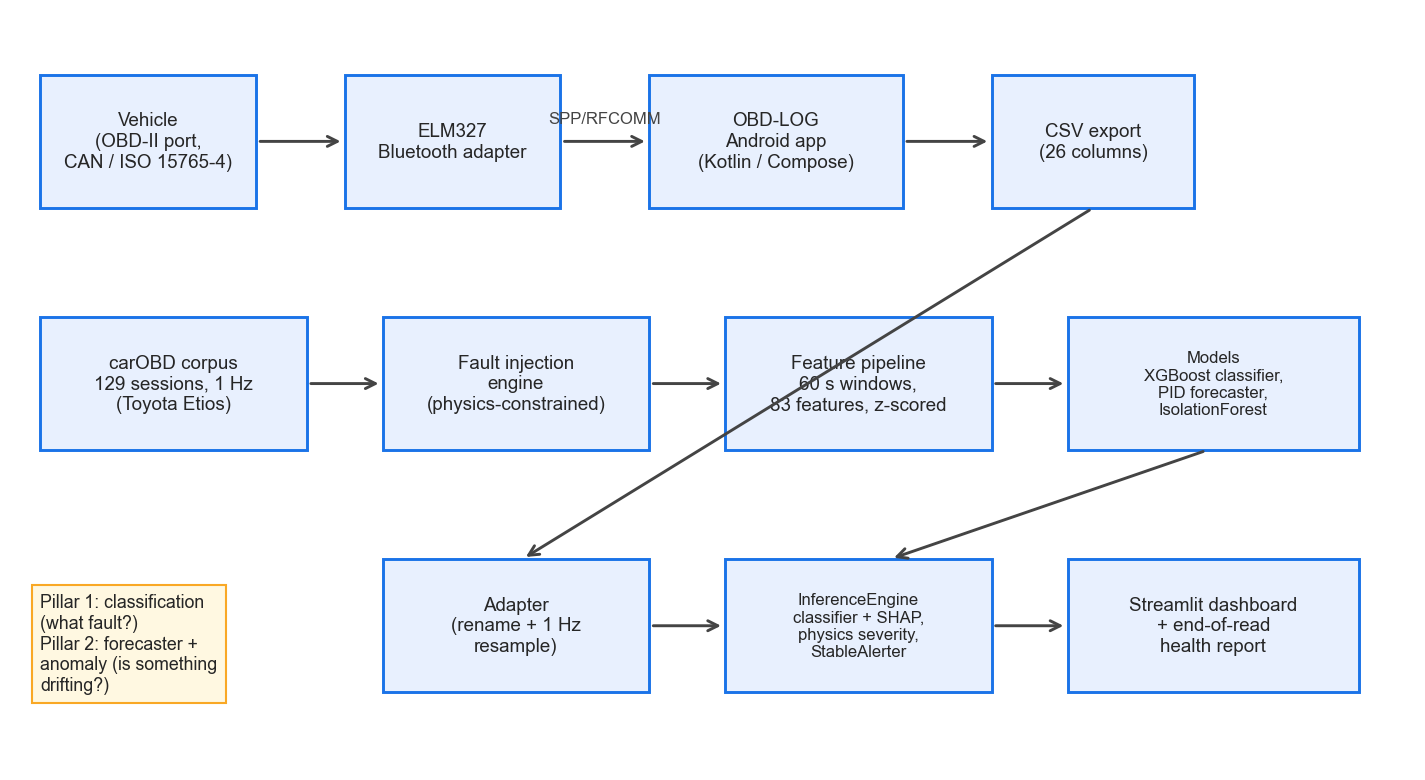
\includegraphics[width=\textwidth]{fig_architecture.png}
  \caption{System architecture. The top row is the acquisition path on the
    vehicle; the middle row is the training pipeline built on the carOBD
    corpus; the bottom row is the inference path that scores recordings and
    drives the dashboard.}
  \label{fig:architecture}
\end{figure}

The analysis side is deliberately organized as two pillars that answer two
different questions. Pillar~1 is the supervised six-class XGBoost classifier:
\emph{if} something is wrong, \emph{which} of the modeled faults does this
window look like? Pillar~2 is the pair of unsupervised safety nets --- a
per-PID forecaster whose prediction residuals flag drift, and a one-class
IsolationForest that scores how far the current window sits from the healthy
manifold. Pillar~2 exists because Pillar~1 can only name faults it was
trained on; a real engine is under no obligation to fail in one of our four
ways.

Both pillars consume the same feature pipeline and the same per-vehicle
baseline normalization, so a single calibration step (recording a few
minutes of healthy driving) adapts the whole stack to a new car. Everything
runs offline on a laptop; the live demo needs no network connection.

\subsection{Data Collection --- the OBD-LOG Android App}
\label{sec:android}

Public data covers the training side, but deploying against real cars
required our own acquisition tool, so we wrote one. OBD-LOG is a native
Android app in Kotlin with a Jetpack Compose / Material~3 interface. It
connects to any ELM327-compatible adapter over Bluetooth Classic
(SPP/RFCOMM), initializes it with the standard AT sequence (reset, echo off,
linefeeds off, spaces off, automatic protocol detection), asks the ECU which
PIDs it actually supports via the 0100/0120/0140 support bitmasks, and then
polls the supported set in a round-robin loop, appending one CSV row per
sweep. The full logger and PID-table sources are reproduced in
Appendix~\ref{app:android}. Our test vehicle throughout was a 2015 Toyota
Yaris, which talks ISO 15765-4 CAN~\cite{iso15765}.

The app's central design decision is a three-tier PID list, because polling
is serial: every extra PID costs sample rate for all of them. Tier~1
(``Core'') carries the nine highest fault-signal channels --- RPM, load,
MAP, MAF, coolant, intake air temperature, both fuel trims, and timing
advance. Tier~2 (``Extended'') adds context: speed, throttle, commanded
equivalence ratio, module voltage, barometric pressure. Tier~3 (``Full'')
adds the remaining niche channels through to catalyst temperatures, kept
mainly for throughput testing. We measured the trade-off directly on the
Yaris at parked idle, and Table~\ref{tab:pollrate} shows why the tiers
exist: tripling the PID count costs two-thirds of the sample rate.

\begin{table}[H]
  \centering
  \caption{Measured poll rate versus polled PID count (2015 Toyota Yaris,
    ELM327 Bluetooth clone, parked idle).}
  \label{tab:pollrate}
  \begin{tabular}{lccc}
    \toprule
    Capture mode & PIDs polled & Measured rate & Rows in test capture\\
    \midrule
    Core     & 7  & 1.10\,Hz & 124\\
    Extended & 12 & 0.64\,Hz & 121\\
    Full     & 21 & 0.37\,Hz & 65\\
    \bottomrule
  \end{tabular}
\end{table}

The three captures in Table~\ref{tab:pollrate} were all successful
end-to-end runs: connect, init, detect, log, export. They also produced the
project's single most consequential hardware finding: the Yaris returned
\texttt{NO DATA} for PID 010B on every request. The car has no MAP sensor
--- it is a MAF-based engine --- so the \texttt{INTAKE\_MANIFOLD\_PRESSURE}
column is empty in every capture. We added MAF (PID 0110) to the Core tier
in response, and Section~\ref{sec:dashboard} describes how the analysis side
was redesigned to survive exactly this kind of per-vehicle sensor absence.

Each CSV carries 26 columns: \texttt{timestamp\_ms} (epoch milliseconds),
\texttt{datetime} (human-readable), and all 24 defined PIDs in fixed order.
Unpolled or unsupported PIDs are written as empty cells rather than dropped,
so every capture has an identical schema regardless of mode --- a property
the downstream adapter relies on. The interface is four screens behind a
navigation drawer: \emph{Dashboard} (connection control, live values, start/stop
logging), \emph{Logs} (recorded files with share/export), \emph{Diagnostics}
(the raw ELM327 init log and support-detection output, which proved
invaluable against clone adapters), and \emph{About}.

One improvement is conspicuously absent and deliberately listed as future
work: a session-label text field written into the CSV, so a recording can
declare itself ``baseline'' or ``induced fault X'' without an external
notebook. It is a one-line UI change, and it is exactly what the real-fault
collection protocol will need.

\subsection{Dataset --- carOBD}
\label{sec:dataset}

Training data comes from carOBD~\cite{maranhao_carobd}, a public corpus of
1\,Hz OBD-II logs from a single Toyota Etios 2014 recorded through a
Carloop (ELM327-compatible) device across 27 PIDs. The corpus spans five
session families: parked idle (\texttt{idle}, 47 files), a recurring
work--home commute (\texttt{live}, 39), highway-style driving
(\texttt{drive}, 13), long trips (\texttt{long}, 12), and low-speed
university-campus driving (\texttt{ufpe}, 18). After the parsing repair
described next, the working corpus is 129 files, 304{,}299 rows, roughly
84.5 hours of driving.

\subsubsection{The trailing-comma discovery}
\label{sec:trailingcomma}

Our Week-1 audit checked every file against physical bounds for four
signature PIDs and produced an alarming result: 120 of 129 files carried
timing-advance values between 30$^{\circ}$ and 776$^{\circ}$, where the
OBD-II encoding cannot exceed $\pm$64$^{\circ}$~\cite{saej1979}. We
initially concluded the files used inconsistent logger firmware and cut the
working set to the 9 clean files --- about 4.4 hours of data --- which is
painfully little for a six-class problem.

The real cause was one character per line. The affected files end every data
row with a trailing comma, so each row parses to 28 fields against 27 header
names. Given that mismatch, \texttt{pandas.read\_csv} silently resolves the
difference by promoting the first column to the row index --- and thereby
shifts \emph{every} column one position left. Coolant temperature reads
fuel-trim values. Timing advance reads catalyst temperature, which is
exactly why we saw ``timing'' of 300--776$^{\circ}$: those are plausible
catalyst temperatures in $^{\circ}$C. The data was never corrupt. The parse
was.

\begin{figure}[H]
  \centering
  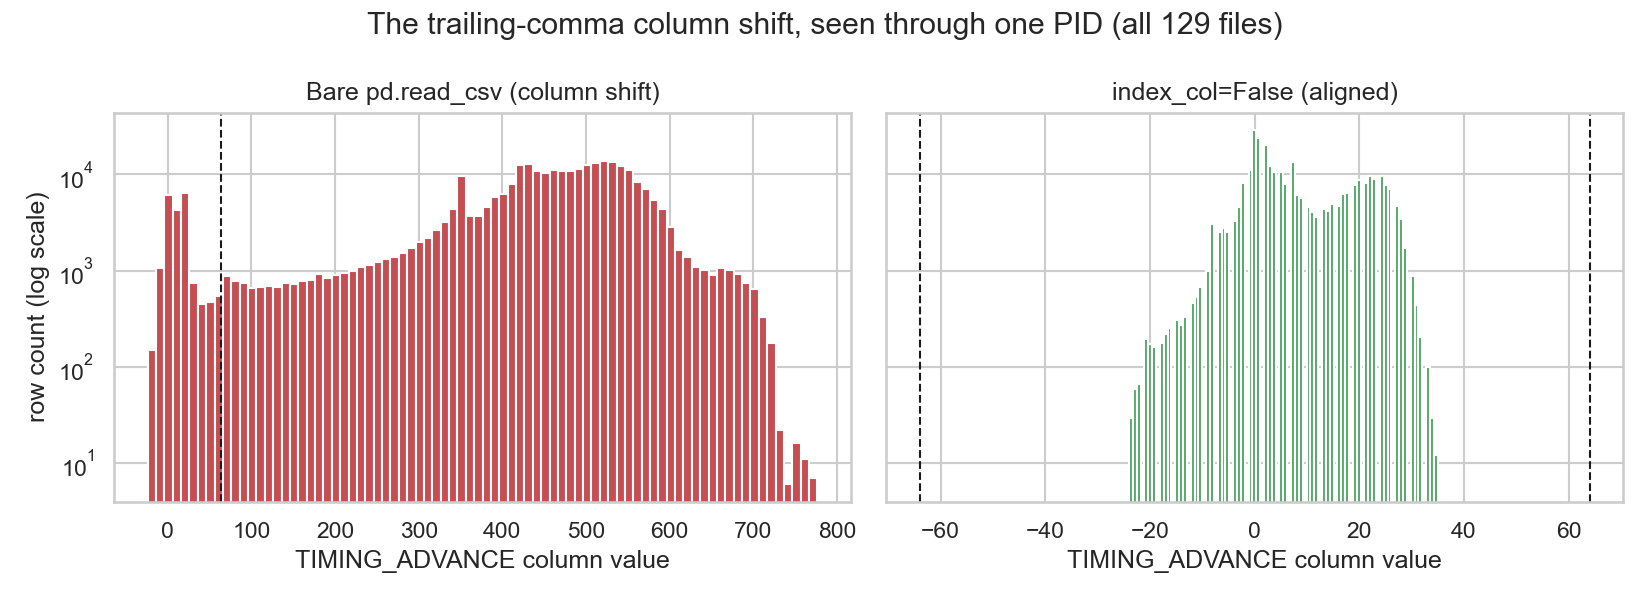
\includegraphics[width=\textwidth]{fig_timing_fix.png}
  \caption{The column-shift defect seen through one PID. Left: under a bare
    \texttt{read\_csv}, the TIMING\_ADVANCE column contains a large
    population far outside the $\pm$64$^{\circ}$ OBD-II bound (dashed
    lines), peaking at 776.6$^{\circ}$ --- catalyst temperatures wearing the
    wrong column name. Right: with \texttt{index\_col=False} the same files
    yield $-24^{\circ}$ to $+35^{\circ}$, entirely inside the physical
    range. Note the logarithmic count axis.}
  \label{fig:timingfix}
\end{figure}

The repair has three parts, and all three stay in the codebase. First,
\texttt{index\_col=False} tells the parser never to promote a column, which
aligns all 27 columns in every file. Second, a numeric coercion pass
converts stray non-numeric cells (one file hides a lone space character in
the intake-air-temperature column) to missing values instead of letting one
bad cell change a whole column's type. Third --- the part we consider
non-negotiable --- a physical-bounds guard re-checks the four signature PIDs
on every load and raises a loud error on violation, so any future
misalignment fails at the loader instead of entering training as scrambled
``healthy'' data. A regression test locks the guard in place. The fix took
the usable corpus from 9 files ($\sim$4.4\,h) to 129 files
($\sim$84.5\,h), a 19$\times$ expansion, and Figure~\ref{fig:timingfix} is
the before/after evidence.

Frankly, this bug taught us more about data engineering than any lecture
could: the failure mode was silent, the symptom appeared two layers away
from the cause, and the wrong-but-plausible explanation (bad firmware)
survived for weeks because it fit the evidence we had.

\subsubsection{Working PID set}

Four of the 27 channels are dead in this corpus and are dropped at load
time: the commanded equivalence ratio is always zero (the Etios ECU does not
report it), the two MIL counters are always zero (healthy car, lamp never
lit), and warm-ups-since-codes-cleared is pinned at the OBD sentinel 255.
Of the remaining channels, 14 form the working feature set
(\texttt{USEFUL\_PIDS}): RPM, speed, throttle, engine load, coolant
temperature, both fuel trims, MAP, both accelerator-pedal channels,
commanded throttle, intake air temperature, timing advance, and control
module voltage.

\subsection{Fault Injection Engine}
\label{sec:injector}

The injection engine is the project's most technically serious contribution,
and it exists for a blunt reason: the faults we want to detect are not for
sale in any public dataset, so we had to write them --- without writing
physics fiction. The governing rule, enforced in code, is that the engine
never emits a sensor value that violates engine causality. Fuel trims are
clamped to the OBD-II $\pm$25\,\% range, coolant may not change faster than
1$^{\circ}$C per second (thermal inertia), MAP may not exceed barometric
pressure on a naturally aspirated engine, throttle stays within
0--100\,\%, and timing stays within its normal $-10^{\circ}$ to
$+40^{\circ}$ envelope. The full source is Appendix~\ref{app:python}
Listing~\ref{lst:injector}.

Each of the four fault models encodes a specific mechanical argument.

\textbf{Air system (vacuum leak).} Our first implementation followed the
textbook: a leak means unmetered air, so short-term fuel trim swings
strongly positive. We rejected that model after checking it against the
engine we actually train on. The Etios reports MAP, load, and barometric
pressure but no MAF --- it is a \emph{speed-density} engine, which computes
airflow \emph{from} manifold pressure. On such an engine the MAP sensor
measures the post-leak pressure directly, the ECU recomputes airflow from
it, and fuel largely self-compensates; service literature for MAP-only
engines describes a slightly raised idle as often the only symptom. The
corrected model therefore raises idle RPM (the leak behaves like a
cracked-open throttle blade, about 15\,rpm per unit of leak magnitude,
clamped to a 1{,}500\,rpm idle ceiling), raises idle MAP slightly, raises
calculated load slightly, and applies only a small, idle-gated fuel-trim
bump that washes out entirely off idle. Every effect is weighted by an
idle factor that goes to zero as load rises, because a leak that is 20\,\%
of airflow at idle is noise at wide-open throttle.

\textbf{Fuel system (injector clog / low rail pressure).} Less fuel per
spray cycle produces a chronic lean condition that the ECU corrects. The
detail that matters --- and that a naive injector gets wrong --- is the
division of labor between the two trims. Short-term trim is the fast
corrector: it \emph{leads} during the developing fault. Long-term trim is
the learned correction: it integrates upward and \emph{holds}. Once the
fault stops developing, STFT bleeds back toward zero (still oscillating)
over roughly a 60-second constant while LTFT retains the full offset. Our
\texttt{\_steady\_state\_trim} helper implements exactly this handoff, so a
developed fuel fault presents as high LTFT with near-zero mean STFT --- the
relationship a real adaptive ECU produces. MAP is deliberately left
untouched: an injector restricts fuel, not air, and that untouched MAP is
what separates a fuel fault from an air fault in feature space. A small
idle-only RPM jitter models the roughness of an unevenly fed engine.

\textbf{Coolant temperature sensor (stuck cold).} The reported temperature
drifts toward a stuck value (default 42$^{\circ}$C), with the
1$^{\circ}$C-per-second clamp applied sample by sample so the trajectory
respects thermal inertia even in step mode. The ECU consequences follow:
timing is retarded in proportion to the perceived cold deficit (up to
5$^{\circ}$), and --- the consequence our first version missed entirely ---
the ECU holds cold-start enrichment because it believes the engine never
warmed up, so once closed-loop operation is reached the fuel trims go
\emph{negative} (rich), delivered through the same STFT-to-LTFT handoff. A
stuck-cold sensor without the rich bias would be a signature no real car
produces.

\textbf{Throttle position sensor (potentiometer wear).} The reported
throttle angle drifts multiplicatively (default full-ramp factor 1.35), but
only on rows where the accelerator pedal exceeds 10\,\% --- a worn
potentiometer track is not loaded at closed throttle, so idle rows stay
clean. The commanded-throttle channel is deliberately left unchanged, which
makes reported-versus-commanded divergence a second, independent signal on
top of the throttle-to-pedal ratio.

Two properties hold across all four models. Degradation is a \emph{ramp}:
severity rises linearly from zero at a configurable onset (default 40\,\%
into the session) over a configurable width (default 15\,\%), then holds
--- modeling gradual wear, with step mode as the one-row limiting case.
And every injection is reproducible: the random seed, onset index, ramp
length, magnitude, and noise level are stored in the output's metadata, so
any training window can be traced to exactly the parameters that produced
it.

One threat looms over all of this, and we measured it instead of waving at
it. The classifier learns to invert the injector; the injector defines the
answer key. If the model merely memorizes our coefficients, its scores are
meaningless for any fault we did not author. The withheld-configuration
experiment in Section~\ref{sec:evalmethod} trains on one full parameter
configuration and tests on a shifted one --- different magnitudes, onset,
ramp width, and noise --- and the observed macro-F1 gap is 0.033. Small,
but not zero, and we report every synthetic score in this book with that
caveat attached: they are a self-consistency floor, not field detection.

\subsection{Feature Engineering}
\label{sec:features}

The 60-second window and 10-second stride are not arbitrary. Sixty seconds
is long enough to capture the slow signatures the faults live in --- a fuel
trim settling to a new level, a coolant curve failing to rise --- while
staying short enough that a driver's state (idling, accelerating, cruising)
is roughly constant across the window, which keeps the regime features
meaningful. The 10-second stride means consecutive windows overlap by 50
seconds, giving a sixfold data-augmentation effect over non-overlapping
windows. That overlap is also precisely why the evaluation of
Section~\ref{sec:evalmethod} must split by session: two windows ten seconds
apart are almost the same window, and letting one train while the other
tests is self-examination, not generalization.

The classifier never sees raw rows. Each 60-second window (stride 10\,s)
is summarized into 83 features in four groups:

\begin{itemize}
  \item \textbf{Per-PID statistics (70).} For each of the 14 working PIDs:
    mean, standard deviation, minimum, maximum, and first-to-last delta.
  \item \textbf{Cross-PID ratios (4).} \texttt{THROTTLE\_TO\_PEDAL\_RATIO}
    (the TPS fault's home signal, computed as the median per-row ratio over
    pedal-active rows only, because the mean ratio explodes at idle);
    \texttt{MAP\_PER\_THROTTLE} (airflow sanity, open-throttle rows only);
    \texttt{FUEL\_TRIM\_DIVERGENCE} ($\mathrm{LTFT} - \mathrm{STFT}$, which
    directly encodes the handoff state); and
    \texttt{THROTTLE\_CMD\_ACTUAL\_DELTA} (reported minus commanded
    throttle).
  \item \textbf{Trajectory features (4).} \texttt{COOLANT\_WARMUP\_RATE} in
    $^{\circ}$C/min (a stuck sensor warms at zero rate);
    \texttt{FUEL\_LOOP\_ACTIVE} (closed-loop indicator);
    \texttt{RPM\_IDLE\_DRIFT} (idle stability);
    \texttt{TIMING\_VS\_TEMP} (timing deviation from the temperature-implied
    norm).
  \item \textbf{Operating-regime one-hots (5).} cold\_start / warmup /
    idle / accel / cruise, detected from coolant, speed, and pedal
    variance, so the model can condition every other feature on context.
\end{itemize}

The representation's load-bearing property is what happens \emph{after}
extraction: every feature is z-scored against the source vehicle's own
healthy baseline (mean and standard deviation fitted on designated healthy
data). The model never reasons about ``LTFT $= 15\,\%$''; it reasons about
``LTFT is 4$\sigma$ above normal \emph{for this car}.'' Raw values differ
between a 2014 Etios and a 2015 Yaris for perfectly healthy reasons ---
deviations from each car's own normal are comparable. This single decision
is the cross-vehicle transfer mechanism, and it reduces adapting the system
to a new vehicle to fitting one scaler on a few minutes of healthy driving.

\subsection{Model Development}
\label{sec:models}

\textbf{XGBoost classifier (Pillar 1).} The production classifier is an
XGBoost~\cite{chen2016} multi-class model over the 83 normalized features:
six classes (healthy, cold\_start, air\_system, fuel\_system,
coolant\_temp\_sensor, throttle\_position\_sensor), 300 trees of depth 6,
learning rate 0.1, 80\,\% row and column subsampling, and the
\texttt{multi:softprob} objective so downstream consumers get full
per-class probabilities. Two weighting mechanisms shape training: samples
are weighted inversely to class frequency (cold-start windows are scarce at
about 5\,\%), and fuel-system samples carry an additional 0.5 down-weight
--- a correction added when that class over-fired (precision 0.457) in an
early build. Training source: Appendix~\ref{app:python}
Listing~\ref{lst:xgb}.

\textbf{Random Forest baseline --- kept as a warning label.} Before XGBoost
we trained a Random Forest~\cite{breiman2001} on an earlier five-class
version of the task, and it scored a macro-F1 of exactly 1.000 on the
held-out sessions. We kept that number in the repository deliberately. A
perfect score does not mean the problem is solved; it means the synthetic
task, as then configured, was trivially memorizable. The subsequent drop to
0.962 when we hardened the physics (the speed-density rewrite, the trim
handoff, magnitude jitter) is evidence of rigor, not regression --- the
task got harder because it got more honest.

\textbf{PID forecaster (Pillar 2a).} Four XGBoost regressors, one per fault
class's key channel, each predicting the \emph{change} in that channel
(in $\sigma$ units) 60 seconds ahead: coolant temperature, MAP, the
throttle-to-pedal ratio, and LTFT. Trained on healthy windows only. The
residual between forecast and arrival is a model-agnostic drift signal: a
sensor moving in a way the healthy dynamics cannot explain is suspicious
regardless of which fault class it resembles. Each regressor is judged
against the persistence baseline (``predict no change''), and one of the
four fails that test: LTFT forecasting is 2.3$\times$ \emph{worse} than
persistence (Section~\ref{sec:forecastresults}). We document that failure
rather than hide it, because LTFT is the single most diagnostic fuel-fault
channel, and knowing the forecaster cannot anticipate it is operationally
relevant.

\textbf{IsolationForest anomaly detector (Pillar 2b).} A one-class
IsolationForest~\cite{liu2008} trained on healthy windows over a 12-feature
subset, emitting a 0--1 out-of-distribution score. Its test AUC of 0.69 is
weak, and we say so; it is included as a complement to the classifier
because it is the only component with any chance of reacting to a fault
class we did not model.

The SHAP panel deserves a concrete example, because explanation is a real
requirement in a diagnostic tool and not a decoration. When the classifier
flags a fuel-system fault, the panel does not just show the label; it shows
that (say) the long-term fuel trim mean contributed $+0.43$ toward that
class, the fuel-trim divergence feature contributed $+0.21$, and the
unchanged MAP contributed a smaller push away from air-system. A mechanic
reading that does not need to trust the model on faith --- the explanation
names the two sensors a fuel fault should move and confirms the one it
should not, and those are checkable claims. When the same panel instead
attributes a prediction mostly to a regime one-hot or a voltage feature,
that is a signal to distrust the call. Making the model's reasoning legible
is what lets a human catch the model's mistakes, and it is why we pay the
cost of exact TreeExplainer computation on every scored window rather than
shipping a bare label.

\textbf{StableAlerter (temporal vote).} Raw per-window labels flicker, and
a dashboard that flickers trains its user to ignore it. A fault alert
therefore requires a majority across a three-window vote with hysteresis
before it is raised or cleared. Two hard rules ride on top: non-fault
labels (healthy, cold\_start, warming-up) can never raise a fault alert,
and any label declared Untested for this vehicle is rewritten to healthy
\emph{before} it enters the vote --- an untrustworthy prediction should not
accumulate votes toward an alarm.

\subsection{Dashboard}
\label{sec:dashboard}

The operator-facing layer is a Streamlit~\cite{streamlit} application that
replays recorded CSVs at 1--50$\times$ speed or attaches to a live ELM327
stream. Top to bottom it renders: a full-width status banner (state,
confidence, session time); a fault severity strip showing per-fault
physics-derived severity bars --- severity comes from closed-form formulas
over the features, not from the forecaster, after the forecaster produced
phantom 17--27\,\% severities on healthy cars; live sparklines for four key
PIDs; a SHAP top-contributors panel translating feature attributions into
workshop vocabulary; and a time-stamped alert log fed by the StableAlerter
and the deterministic cold-start rule checker.

When a replayed file ends, the dashboard renders its primary output: the
end-of-read health report. The report treats the first 20\,\% of the
recording as the vehicle's own baseline and excludes it from the verdict
(scoring the baseline against itself is circular). Over the remaining
windows it computes, per fault, the share of windows won and the 95th
percentile of physics severity. A fault is DETECTED only if it wins at
least 40\,\% of evaluable windows \emph{and} carries material severity; a
fault that dominates labels at approximately zero severity is reported
INCONCLUSIVE, because that combination is the signature of a feature
artifact, not physics. Fewer than 10 evaluable windows yields INSUFFICIENT
DATA rather than a verdict. Every report carries its caveats in the
rendered output, including the one that matters most: this design detects a
fault that \emph{develops during the recording}; a fault already present at
key-on becomes the baseline and reads as normal.

The report's Untested machinery deserves its own paragraph, because a real
failure created it. Different cars expose different PIDs, and each fault
class declares the PIDs its primary signature requires
(Appendix~\ref{app:python} Listing~\ref{lst:pidavail}): air\_system
requires MAP; TPS requires throttle, commanded throttle, \emph{and both}
pedal channels; and so on. When we first scored our healthy MAF-based Yaris
--- a car with no MAP sensor --- the pipeline filled the missing MAP
features with the training vehicle's baseline values, the classifier read
that fabricated flatness as a massive deviation, and the dashboard
announced a 97\,\% air-system fault on a healthy car. The false positive,
not theory, drove the redesign: a missing PID now yields NaN features
(which XGBoost routes through learned default splits), the affected fault
class is marked Untested for the whole session, its label is suppressed
from alerting, and the end-of-read report prints ``UNTESTED --- PID
unavailable'' where a score would have been. Fabricated sensor values
produce confident wrong answers; refusing to score is the honest
alternative, and Chapter~\ref{ch:results} shows it working on the same car
that broke the first version.
